


Receber uma base de dados não estruturada;
kk


Desenvolveu-se uma
Metodologia que conecta 
Metodologia que agrupa segmentos de ata por tópico.


A metodologia utilizada nesse trabalho: 
\begin{itemize}
	\item Conecta as técnicas de segmentação textual aos modelos de extração de tópicos 
	\item Gera um estrutura derivada de um \textit{corpus} não estruturado.
	% \item Descobre e identifica variáveis latentes pa
	\item Utiliza variáveis latentes em conjunto com técnicas de Recuperação de Informação.
\end{itemize}


Essa organização permite
que técnicas de Recuperação de Informação expandam o espaço de busca além do conjunto


Expandir o espaço de busca; 




% \begin{frame}{Análise dos Resultados}



% \begin{figure}[!ht] \centering     %%% not \center

	% Performance geral dos algoritmos de segmentação textual. 

		% 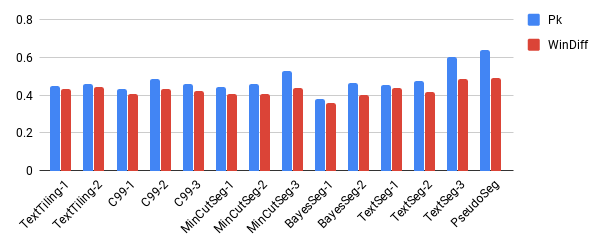
\includegraphics[width=.82\textwidth]{images/graficos/resumo-wd-pk.png}	
		% \label{fig:resumo-wd-pka}
		% 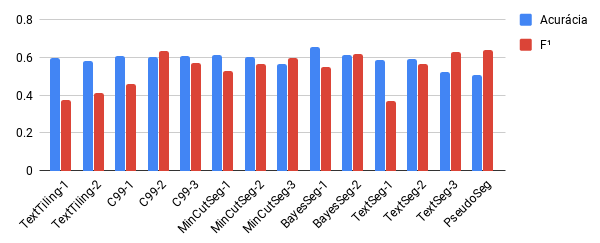
\includegraphics[width=.82\textwidth]{images/graficos/resumo-tradicionais.png}	
		% \label{fig:resumo-tradicionaisa}

	% \label{fig:resumo-segmentadores}
% \end{figure}



% \end{frame}


		\includegraphics[trim={ 0 235 0 16 },clip,page=1,width=0.73\textwidth]{images/distribuicao.pdf}
tela-principal-2-1.png
ficando os demais disponíveis para exploração pelo usuário.

Os tópicos mais similares à consulta ficam disponíveis para exploração.


Busca exploratória pelos tópicos mais similares à consulta.







O módulo de consulta aproveita a estrutura de dados interna para recuperar informações

Usa-se o modelo de espaço vetorial para ranquear os tópicos.








incorporar conhecimento de domínio aos dados












com isso é possivel identificar em cada ata

com isso é possível identificar trechos que tradam de um assunto
com isso é possível identificar os assuntos tratados em uma ata bem como sua 

com isso é possível identificar nas atas os trechos que tradam de um assunto


com isso é possível identificar os assuntos tratados em uma ata. 



Essa abordagem permite a expansão do espaço de busca além do conjunto de termos original de cada segmento, e a identificação de trechos mais relevantes à consulta.






\nblock{ Estrutura mais organizada} {
	\begin{itemize}
		\item  Segmentos agrupados por tópico.
		\item  Segmentos acrescidos de novos atributos (tópicos)
	\end{itemize}
}




\begin{center}
    \begin{minipage}{0.5\textwidth}
		\begin{description} \tiny
			\item[DT] Discordo Totalmente
			\item[DP] Discordo Parcialmente
			\item[NCND] Não Concordo Nem Discordo
			\item[CP] Concordo Parcialmente
			\item[CT] Concordo Totalmente
		\end{description}
    \end{minipage}
  \end{center}



\begin{center}
    \begin{minipage}{0.5\textwidth}
		\begin{description} \tiny
			\item[N] Nenhum
			\item[P] Poucos
			\item[NMNP] Nem Muitos nem Poucos
			\item[M] Muitos
			\item[T] Todos
		\end{description}
    \end{minipage}
  \end{center}



\begin{figure}[!h] \centering     %%% not \center
%	\subfigure{ \label{fig:kmeans}
		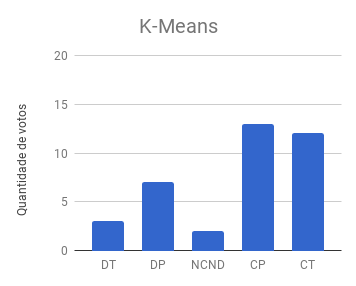
\includegraphics[width=.31\textwidth]{conteudo/capitulos/figs/figuras-experimento/Q1-KMeans.png}
%	}	
%	\subfigure{ \label{fig:lda}
		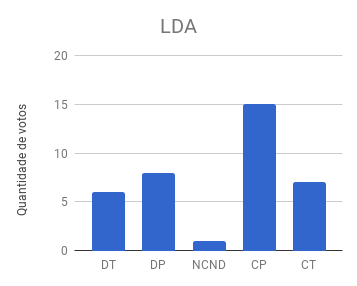
\includegraphics[width=.31\textwidth]{conteudo/capitulos/figs/figuras-experimento/Q1-LDA.png}
%	}
%	\subfigure{ \label{fig:plsa}
		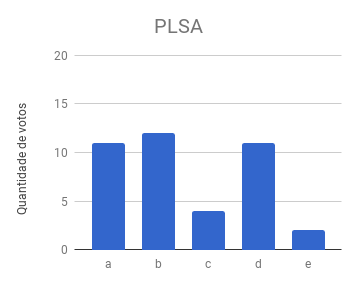
\includegraphics[width=.31\textwidth]{conteudo/capitulos/figs/figuras-experimento/Q1-PLSA.png}
%	} 
	\caption{Contagem de respostas referente a primeira questão cujo enunciado foi:\textit{``Todos os trechos apresentados compartilham um mesmo assunto.''}. O eixo vertical indica a frequência das alternativas representadas no eixo horizontal. }
	\label{fig:Q1}
\end{figure}












\begin{figure}[!h]
	\centering     %%% not \center

	\subfigure[a]{ \label{fig:a}
		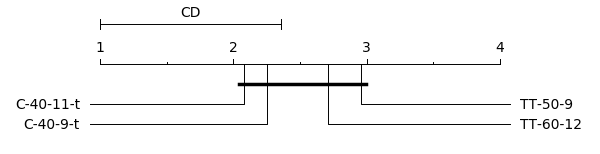
\includegraphics[width=70mm]{conteudo/capitulos/figs/CDs/WinDiff.png} }	
	\subfigure[b]{ \label{fig:b}
		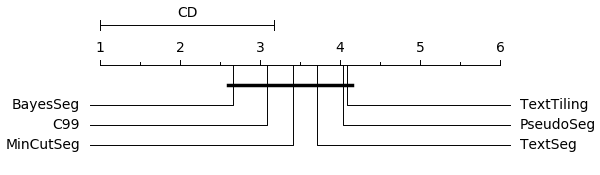
\includegraphics[width=70mm]{conteudo/capitulos/figs/CDs/Pk.png} }
	\subfigure[c]{ \label{fig:c}
		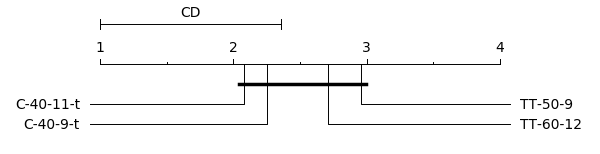
\includegraphics[width=70mm]{conteudo/capitulos/figs/CDs/Acuracy.png}}
	\subfigure[d]{ \label{fig:d}
		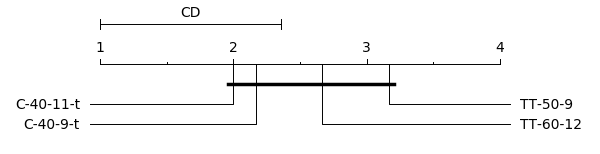
\includegraphics[width=75mm]{conteudo/capitulos/figs/CDs/Precision.png}}
	\subfigure[e]{ \label{fig:e}
		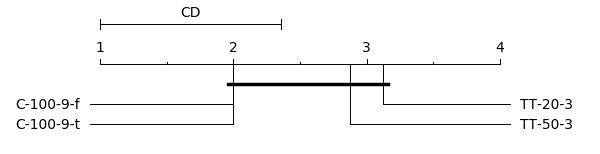
\includegraphics[width=70mm]{conteudo/capitulos/figs/CDs/Recall.png}}
	\subfigure[f]{ \label{fig:f}
		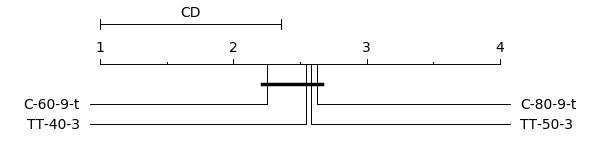
\includegraphics[width=70mm]{conteudo/capitulos/figs/CDs/F1.png}}

		\caption{Diagramas de Diferença Crítica sobre \textit{ranking} dos algoritmos de segmentação baseados em coesão léxica de acordo com valores de \textit{WindowDiff}, $P_k$, Acurácia, Precisão, Revocação e $F^1$.}
	\label{fig:CDs}
\end{figure}







  \begin{center}
	\begin{figure}[h!]

		\includegraphics[trim={ 0 235 0 0 },clip,page=1,width=\textwidth]{conteudo/capitulos/figs/doc-em-png/distribuicao.pdf}

	\end{figure}
\end{center}


\label{fig:distribuicao-ata}

\caption{Distribuição de tópicos em uma ata real. Cada tópico é representado por uma região colorida. Abaixo estão os descritores identificados pela cor do respectivo tópico. Os nomes de pessoas foram ocultados por não expressarem significado nesse trabalho.}





Informações contidas em grandes quantidades de texto;
Grandes volumes de texto com conteúdo irrelevante;
Documentos desestruturados;
Dificuldade em resgatar essas informações manualmente;


	\item Uma atas registra vários assuntos;

Motivação:
\begin{itemize}
	\item São fontes de consulta e utilizadas como referência e apoio a decisões; 
	\item Um assunto pode ser discutido diversas vezes em reuniões diferentes;
	\item É desejável recuperar um histórico dessas decisões ao longo do tempo;
	\item Necessidade de ferramentas automáticas;
\end{itemize}

Motivação:


Atas de reunião registram os assuntos tratados  como base de dados


\item Contém segmentos de texto com assuntos relativamente independentes; 



- Incapacidade humana em gerenciar grandes volumes de documentos;








Fiz um roteiro com:
Motivação
Objetivos
Proposta
Resultados
e Conclusão


acho que é esse roteiro mesmo
mas tipo
os "trabalhos relacionados"
meio que vão aparecer na motivação
pq vc vai falar que tem alguns estudos que segmentam determinados tipos de texto
mas não o que vc vai trabalhar lá em específico





hora que for explicar abordagem proposta
vc vai explicando cada etapa do seu framework
e lá vc vai mostrando a teoria envolvida com cada parte












A literatura apresenta abordagens 


Essa tarefa tem 2 passos principais:
\begin{itemize}
	\item Encontrar pontos onde há transição de assuntos;
	\item Identificar esse assunto;
\end{itemize}







Visão Geral 
imagem segmentação 
imagem documento com tópicos identificados nos segmentos



  % \begin{figure}[!h]
  % \centering
  % 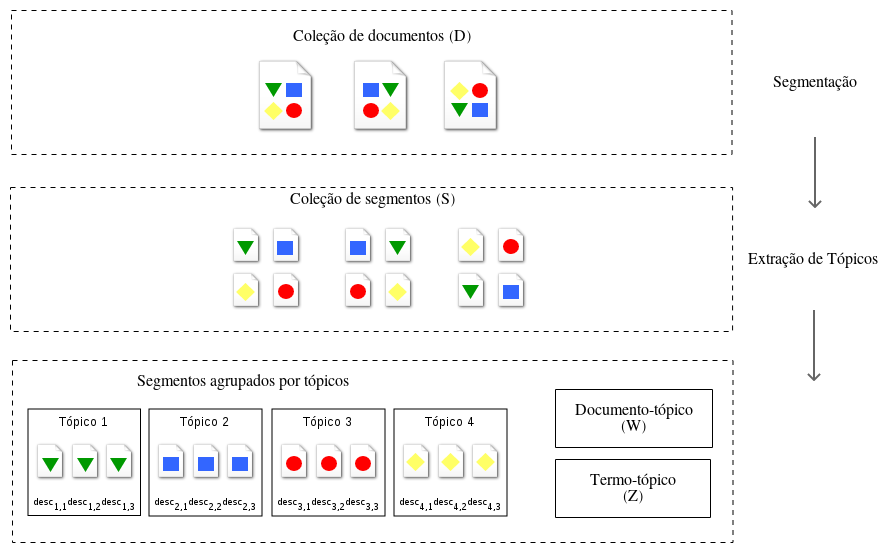
\includegraphics[width=.8\paperwidth]{images/estrutura.png}
  % \caption{Estrutura de dados interna e seu processo de geração.}
% %  \label{fig:#4}
  % \end{figure}





% \nblock{}{
\begin{itemize}
	\item Propor uma solução para identificar, organizar e consultar assuntos registrados em atas de reunião.  
	\item Utilizar técnicas de Segmentação textual em conjunto com modelos de Extração de Tópicos para:
		% \nblock{}{
			\begin{itemize}
	\item Gerar uma estrutura mais organizada que a coleção original.
	\item Utilizar a estrutura latente dos segmentos para Recuperação de Informação. 
		\end{itemize}
		% }
	% \item Dar início a investigação dessa abordagem no contexto de atas de reunião.
\end{itemize}
% }










o objetivo desse trabalho de mestrado é propor o 





desenvolvimento uma ferramenta 


para identificar, organizar e apresentar assuntos registrados em atas de reunião 


utilizando a estrutura latente de documentos segmentados em conjunto com técnicas de recuperação de informação.





% Propor uma solução para encontrar porções de texto relevantes à consulta.






